\documentclass[11pt,oneside]{book}
\usepackage[backend=biber,natbib=true,style=alphabetic,maxbibnames=10]{biblatex}
\addbibresource{/home/nqbh/reference/bib.bib}
\usepackage[utf8]{vietnam}
\usepackage{tocloft}
\renewcommand{\cftsecleader}{\cftdotfill{\cftdotsep}}
\usepackage[colorlinks=true,linkcolor=blue,urlcolor=red,citecolor=magenta]{hyperref}
\usepackage{amsmath,amssymb,amsthm,chemfig,float,graphicx,mathtools,multicol,soul}
\usepackage[version=4]{mhchem}
\allowdisplaybreaks
\newtheorem{assumption}{Assumption}
\newtheorem{baitoan}{Bài toán}
\newtheorem{cauhoi}{Câu hỏi}
\newtheorem{conjecture}{Conjecture}
\newtheorem{corollary}{Corollary}
\newtheorem{dangtoan}{Dạng toán}
\newtheorem{definition}{Definition}
\newtheorem{dinhly}{Định lý}
\newtheorem{dinhnghia}{Định nghĩa}
\newtheorem{example}{Example}
\newtheorem{goal}{Goal}
\newtheorem{ghichu}{Ghi chú}
\newtheorem{hequa}{Hệ quả}
\newtheorem{hypothesis}{Hypothesis}
\newtheorem{lemma}{Lemma}
\newtheorem{luuy}{Lưu ý}
\newtheorem{muctieu}{Mục tiêu}
\newtheorem{nhanxet}{Nhận xét}
\newtheorem{notation}{Notation}
\newtheorem{note}{Note}
\newtheorem{principle}{Principle}
\newtheorem{problem}{Problem}
\newtheorem{proposition}{Proposition}
\newtheorem{question}{Question}
\newtheorem{quyuoc}{Quy ước}
\newtheorem{remark}{Remark}
\newtheorem{theorem}{Theorem}
\newtheorem{vidu}{Ví dụ}
\usepackage[margin=2cm,footskip=1cm]{geometry}
\def\labelitemii{$\circ$}
\DeclareRobustCommand{\divby}{%
	\mathrel{\vbox{\baselineskip.65ex\lineskiplimit0pt\hbox{.}\hbox{.}\hbox{.}}}%
}

\title{Dạy Trẻ Vùng Quê}
%\title{Some Topics in Elementary STEM \textit{\&} Beyond:\\A Personal, Psychological, \textit{\&} Philosophical Perspective\\\vspace{1cm}\textsf{\Large Vài Vấn Đề Trong STEM Sơ Cấp \& Xa Hơn Thế:\\1 Góc Nhìn Cá Nhân, Tâm Lý Học, \& Triết Học.}}
\author{Nguyễn Quản Bá Hồng\footnote{A Scientist- \& Creative Artist Wannabe. e-mail: {\sf nguyenquanbahong@gmail.com}, website: \url{https://nqbh.github.io}, Ben Tre City, Vietnam.}}
\date{\textsf{Version: \today}}

\begin{document}
\maketitle
\begin{quotation}
	\textit{``In this world, is the destiny of mankind controlled by some transcendental entity or law? Is it like the hand of God hovering above? At least it is true that man has no control, even over his own will. Man takes up the sword in order to shield the small wound in his heart sustained in a far-off time beyond remembrance. Man wields the sword so that he may die smiling in some far-off time beyond perception.''} -- \textsc{Kentaro Miura}, \textit{Berserk}, Vol. 1
	\begin{figure}[H]
		\centering
		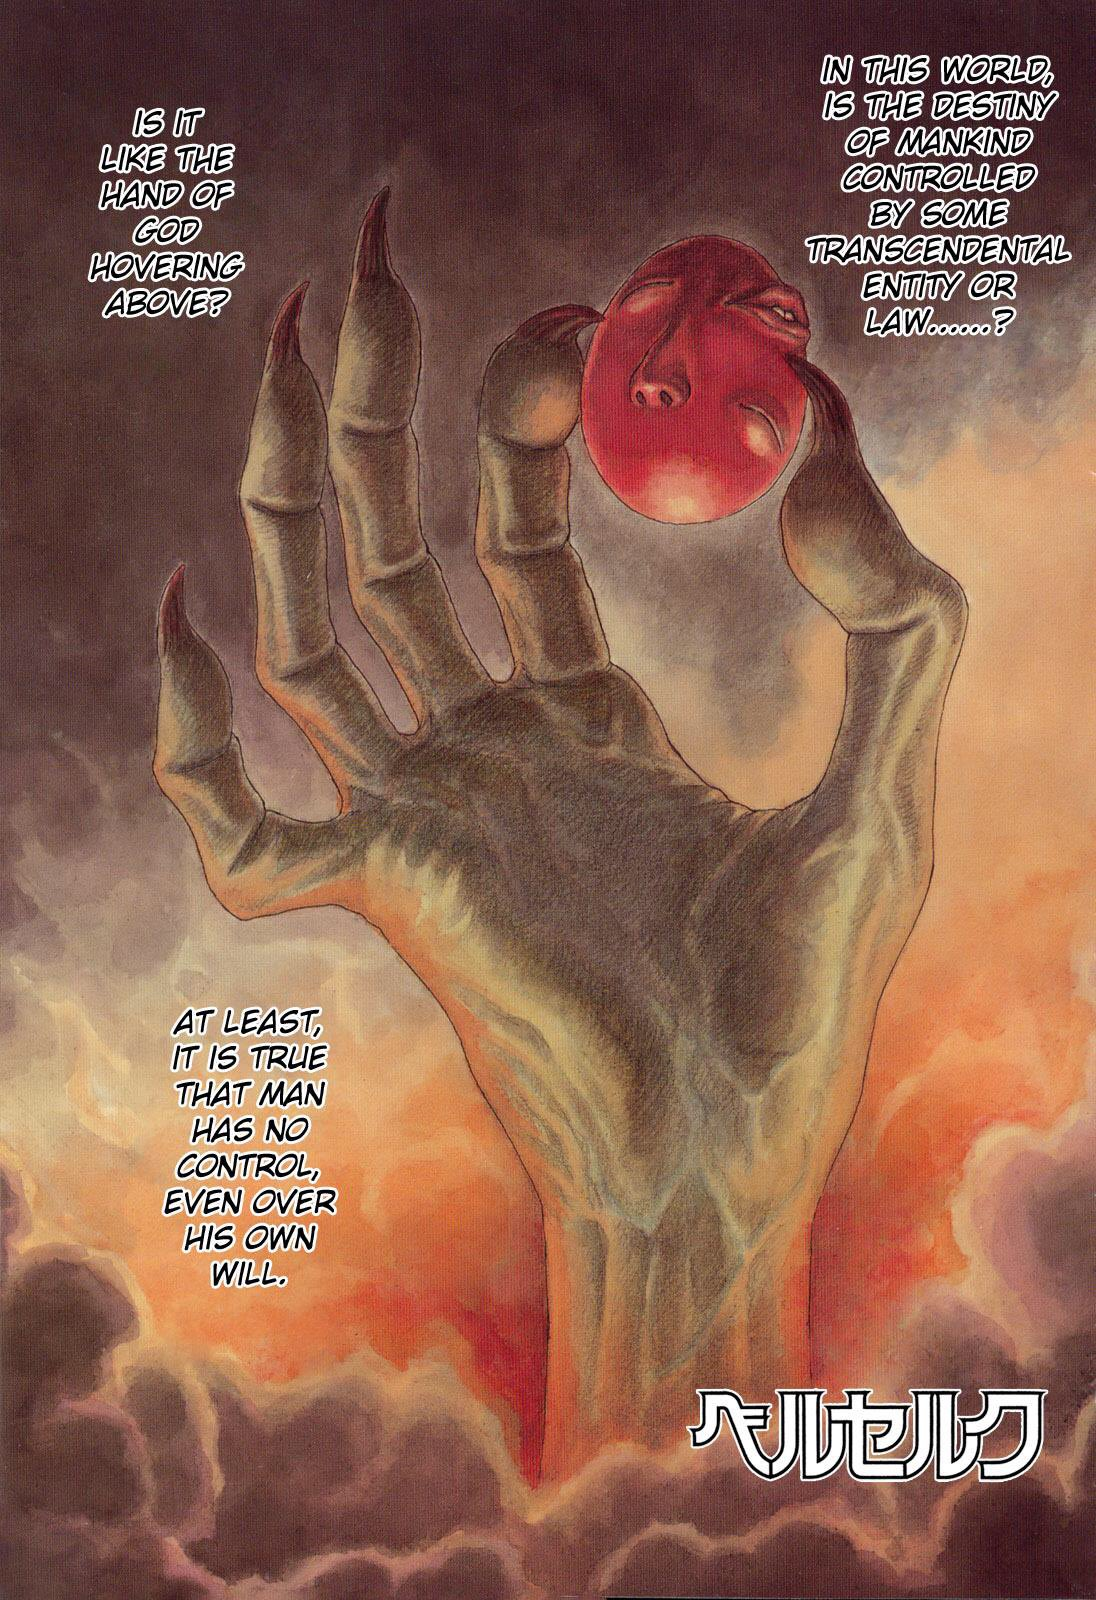
\includegraphics[scale=.15]{Berserk_behelit_color}
		\caption{Berserk, The Hand of God \textit{\&} Behelit.}
	\end{figure}	
	\textit{``Providence may guide a man to meet 1 specific person, even if such guidance eventually leads him to darkness. Man simply cannot forsake the beauty of his own chosen path. When will man learn a way to control his soul?''} – \textsc{Kentaro Miura}, \textit{Berserk}
\end{quotation}
%\hrule
%\begin{multicols}{2}
%	\textit{``What are you doing actually?''} ``I am writing a book.'' \textit{``About what?''} ``I don't know yet.'' \textit{``Huh? You want to write a book but you don't know specifically what to write yet? How can that be?''} ``Everything starts with a sheer will to write, I suppose.'' \textit{``What a joke!''} ``Yeah, let my innocent Infinite Jest \footnote{\textit{Infinite Jest} is the name of a book written by \textsc{David Foster Wallace}, a genius, suicide in ??.} begin.''
%	\columnbreak
%	
%	\textit{``Thực sự là mày đang làm gì vậy?''} ``Tui đang viết 1 cuốn sách.'' \textit{``Về cái gì?''} ``Tui cũng chưa biết nữa.'' \textit{``Hả, mày muốn viết 1 cuốn sách nhưng mày chưa biết viết cụ thể về cái gì? Sao có thể được?''} ``Mọi thứ đều bắt đầu với 1 quyết tâm để viết, tui giả dụ vậy.'' \textit{``Đúng là 1 trò hề!''} ``Ừa, cứ để Trò Hề Vô Hạn nhưng vô hại này bắt đầu.''	
%\end{multicols}
%\hrule
%\noindent
%\begin{verbatim}
%	nqbh@nqbh-mind:~$ reboot
%\end{verbatim}

Tui dự định viết ghi chú này từ cuối năm 2020, cho bản thân là chính (self-grown?), chứ tui không viết để thể hiện hoặc sẽ viết vì mục đích thể hiện cả. Trong quá khứ tui đã nhiều lần làm thế rồi, nên bây giờ \& từ giờ trở đi tui thấy nó thật vô nghĩa \& tui biết vậy. Đơn giản là nếu chỉ để thể hiện như 1 con ngựa non háo đá, tui sẽ nhanh chóng nhận ra mình ngu dốt, thiếu chín chắn, thùng rỗng kêu to cỡ nào rồi lại tự nhục, rồi xóa, rồi kiếm 1 cái gì khác để thể hiện, rồi lại tự nhận thức được rồi nhục, rồi lại tự xóa. Cái vòng thể hiện-nhục-thể hiện-nhục lẩn quẩn cứ lặp đi lặp lại nếu tui mãi không phát triển nhận thức, nên tui sẽ cắt nó ngay từ đầu. Trong hơn 3 năm qua, kể từ cuối năm 2020 -- lần nói chuyện cuối cùng với thầy Quí - thầy dạy Toán cấp 3 của tui, đến nay, đầu năm 2024, có nhiều điều đã thay đổi trong cách nhìn của tui về hành vi, mục đích, các lựa chọn của bản thân \& quan trọng hơn là những cách nhìn mới về cuộc sống.

Nói thật tui chả biết phải bắt đầu từ đâu cho đúng cả. Mà ``cho đúng'' có nghĩa là gì hiện tui cũng không rõ \& đương nhiên là chưa thể làm rõ. Có lẽ nên bắt đầu từ các cuộc trò chuyện thường ngày mà tui có. Tui nghĩ đó là cách tự nhiên \& dễ thấm nhất để các điều tui viết tiếp sau trở nên có nghĩa. Tui ép mọi thứ phải có nghĩa vì tui từng mong muốn trở thành 1 nhà toán học, mà 1 trong các nhiệm vụ chính của 1 nhà toán học điển hình là làm có nghĩa các đối tượng nhà toán học đang quan tâm hoặc vừa sáng tạo ra.

\begin{quyuoc}
	Ký hiệu {\rm name[age, personalities]} ám chỉ 1 người tên `name' với tuổi là `age', với (các) tính cách `personalities' đi kèm.
\end{quyuoc}

\begin{quotation}
	H[12], T[12], N[12], $\ldots$ : Sao thầy giỏi vậy mà không dạy chuyên thầy?
	
	\textsc{hồng[28]}: Nói thực là đến tận giờ tui không chắc việc tui dạy chuyên toán có tốt cho học sinh không. Không phải là tui dạy dở, hoặc ít ra tui tự cho bản thân là dư sức dạy kiến thức chuyên, xưa tui định làm khoa học, tức nhà toán học ấy, nên kiến thức toán tui hơi quá dư để dạy toán sơ cấp, tức mấy cái toán cấp 2, cấp 3, chưa tới toán cao cấp ở đại học trở lên, nhưng tiếc là quá thiếu để làm khoa học. Nó cứ lưng lửng kiểu khó chịu ấy.
	
	Nhưng quan trọng là tui biết tính tui: Tui mà dạy chuyên là tui tham lắm. Không phải tham tiền, mà là tham kiểu gần như ép học sinh học mấy kiến thức cao về Toán. Nếu lỡ tui làm cho 1 đứa đam mê quá sâu vào toán mà bỏ gần như tất cả các thứ khác, liệu có tốt cho tương lai bạn đó không, trong khi nhà bạn đó nghèo \& cần tìm 1 công việc để nuôi gia đình trước rồi mới tính tới đam mê hoặc phải đè bẹp cả đam mê để mà sống tốt bằng cách giúp đỡ cha mẹ vượt qua hoàn cảnh khó cảnh khó khăn của gia đình?
	
	Quan trọng hơn là, liệu tui có đủ kiến thức ngoài toán, ngoài khoa học, tức hiểu chuyện, hiểu đời, để đủ trách nhiệm cho việc dạy hay dẫn dắt 1 ai đó lên 1 nền tảng cao hơn không? Hiện tui thấy là không, mà cái gì tui nhắm không lãnh nổi trách nhiệm thì tui sẽ không làm, lùi 1 bước để nhường cho ai đủ sức lãnh để nó đâu ra đấy, thà đưa tiền cho cha mẹ hết để báo hiếu rồi bản thân nghèo chứ không hại 1 ai cả. Ngu ngu dại dại kiểu ấy. Để xem sao.
\end{quotation}




%------------------------------------------------------------------------------%

\printbibliography[heading=bibintoc]

\end{document}